\chapter{Capturing Dominant I/O Activities of an Application by Program Contexts} 
\section{Definition and Extraction of Program Context}
In developing an efficient optimization technique for general I/O workloads,
our key insight was that in most applications, the overall I/O behavior of
applications is decided by a few dominant I/O activities ({\it e.g.}, logging and
flushing in RocksDB).  Moreover, data written by dominant I/O activities tend
to have distinct I/O patterns.  Therefore, if such dominant I/O activities
of applications can be automatically detected and distinguished each other in
an LBA-{\it oblivious} fashion, an optimization technique can be
developed for varying I/O workloads including append-only workloads.

In this dissertation, we argue that a program context can be used to build an
efficient general-purpose classifier of dominant I/O activities.% with different data lifetimes.  
Here, a PC represents an execution path of an application
which invokes write-related system call functions such as {\tt write()} and
{\tt writev()}.  There could be various ways of extracting PCs, but the most
common approach~\cite{PC, PC2} is to represent each PC with its PC signature
which is computed by summing program counter values of all the functions along
the execution path which leads to a write system call.

\begin{figure}[t]
	\centering
	\includegraphics[width=0.8\textwidth]{figure/pcstream/writepath}
	\caption{An illustration of (simplified) execution paths of two dominant I/O activities in RocksDB.}
	\label{fig:iopath}
\end{figure}


In RocksDB, dominant I/O activities include logging, flushing and compaction.
Since these I/O activities are invoked through different function-call paths,
we can easily identify dominant I/O activities of RocksDB using PCs.  For
example, Fig.~\ref{fig:iopath} shows (simplified) execution paths for logging
and compaction in RocksDB.  The sum of program counter values of the execution
path \texttt{WriteImpl()}$\rightarrow$\texttt{WriteToWAL()}$\rightarrow$
\texttt{AddRecord()} is used to represent a PC for the logging activity while
that of the execution path \texttt{Run()}$\rightarrow$
\texttt{ProcessKeyValueCompaction()} $\rightarrow$
\texttt{FinishCompactionFile()} is used for the compaction activity.
In SQLite, there exist two dominant I/O activities which are logging and
managing database tables.  Similar to the RocksDB, SQLite writes log files and
database files using different execution paths.  In GCC, there exist many
dominant I/O activities of creating various types of temporal files and object
files.


%\subsection{Extracting PCs}
As mentioned earlier, a PC signature, which is used as a unique ID of each
program context, is defined to be the sum of program counters along the
execution path of function calls that finally reaches a write-related system
function.  In theory, program counter values in the execution path can be
extracted in a relatively straightforward manner.  Except for inline functions,
every function call involves pushing the address of the next instruction of a
caller as a return address to the stack, followed by pushing a frame pointer
value.  By referring to frame pointers, we can back-track stack frames of a
process and selectively get return addresses for generating a PC signature.
Fig.~\ref{fig:getpc}(a) illustrates a stack of RocksDB corresponding to
Fig.~\ref{fig:iopath}, where return addresses are pushed before calling
\texttt{write()}, \texttt{AddRecord()} and \texttt{WriteToWAL()}.  Since frame
pointer values in the stack hold the addresses of previous frame pointers, we
can easily obtain return addresses and accumulate them to compute a PC signature.  

%For example,
%Fig.~\ref{fig:getpc}(a) shows abstracted execution paths of log data and
%compaction data in RocksDB.  The return addresses are pushed before calling the
%\textsf{\small  write()}, \textsf{\small AddRecord()} and \textsf{\small
%WriteToWAL()} functions.  Fig.~\ref{fig:getpc}(b) illustrates how a PC
%signature is obtained by back-tracking the stack.  Since frame pointer values
%in the stack hold the addresses of previous frame pointers, we can easily
%obtain return addresses and accumulate them to compute a PC signature.  

The frame pointer-based approach for computing a PC signature, however, is not
always possible because modern C/C++ compilers often do not use a frame pointer
for improving the efficiency of register allocation.  One example is a {\tt
-fomit-frame-pointer} option of GCC~\cite{GCC}.  This option enables to use a frame
pointer as a general-purpose register for performance, but makes it difficult for us
to back-track return addresses along the call chains.  

\begin{figure}[t]
	\centering
	%\subfloat[Abstracted execution paths of two I/O activities of RocksDB.]{\includegraphics[width=0.3\textwidth]{figure/writepath}}  
	%\hfill
	\subfloat[with the frame pointer.]{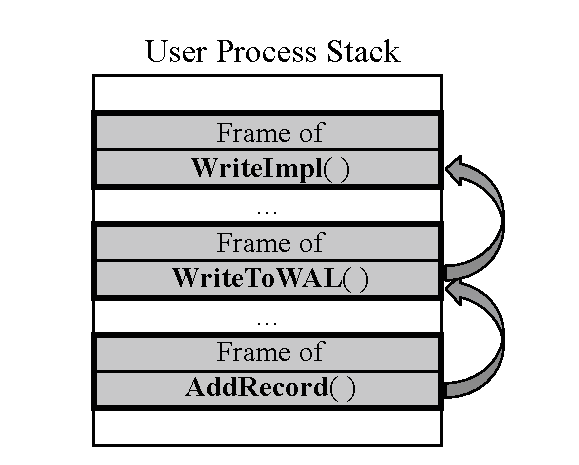
\includegraphics[width=0.4\textwidth]{figure/pcstream/getpc_new1}}
	%\hspace{10pt}
	\subfloat[without the frame pointer.]{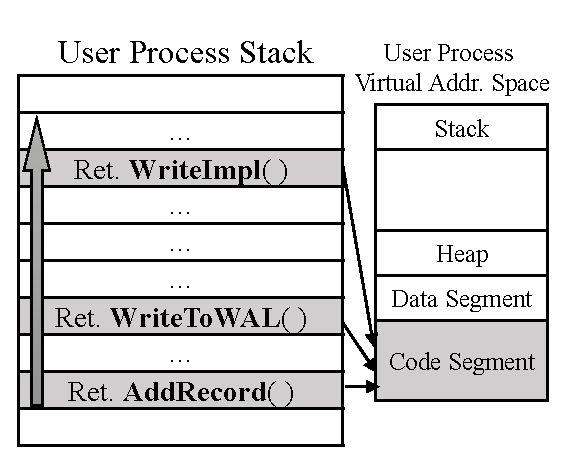
\includegraphics[width=0.445\textwidth]{figure/pcstream/getpc_new2}}
	\caption{Examples of PC extraction methods.}
	%\caption{An example execution path and its PC extraction.} %shane part
	\label{fig:getpc}
\end{figure}

We employ a simple but effective workaround for back-tracking a call stack when
a frame pointer is not available.  When a write system call is made,
we scan every word in the stack
and checks if it belongs to process's code segment.  If the scanned stack word
holds a value within the address range of the code segment, it assumes that it
is a return address.  
Fig.~\ref{fig:getpc}(b) shows the scanning process.
Since scanning the entire stack may takes too long, we stop
the scanning step once a sufficient number of return address candidates are found.
In the current implementation, the scanning process stops early once 
five return address candidates are identified.  
Even though it is quite ad-hoc, this restricted scan is quite effective
in distinguishing different PCs because it is very unlikely that two different PCs
reach the same \texttt{write()} system call through the same execution subpath 
that covers five proceeding function calls. 
In our evaluation on a PC with 3.4 GHz Intel CPU, the overhead of the
restricted scan was almost negligible, taking only 300$\sim$400 $n$sec per
\texttt{write()} system call.

\section{Data Lifetime Patterns of I/O Activities}
In developing automatic stream management technique, our key insight was that in most applications,
(regardless of their I/O workload characteristics)
a few dominant I/O activities exist
and each dominant I/O activity   
represents the application's important I/O context (e.g., for logging or for flushing). 
Furthermore, most dominant I/O activities tend to have distinct data lifetime patterns.
In order to distinguish data by their lifetimes, therefore, 
it is important to effectively distinguish dominant I/O activities from each other.  
For example, in update workloads, 
LBAs alone were effective in separating dominant I/O activities.  
In this dissertation, we argue that a program context is an efficient general-purpose
indicator for separating dominant I/O activities regardless of the type of I/O
workloads.  

\begin{figure}[t]
\centering
	\subfloat[Logging (PC)]{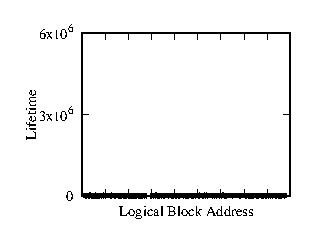
\includegraphics[width=0.4\textwidth]{figure/pcstream_/type_1}} % data from 4/03031953 
	\hspace{10pt}
	\subfloat[Logging (manual)]{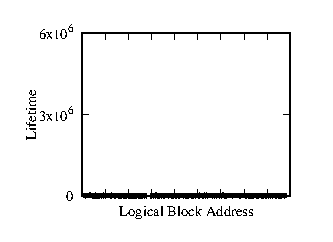
\includegraphics[width=0.4\textwidth]{figure/pcstream_/pcID_2}}
	 \\
	\subfloat[Flushing (PC)] {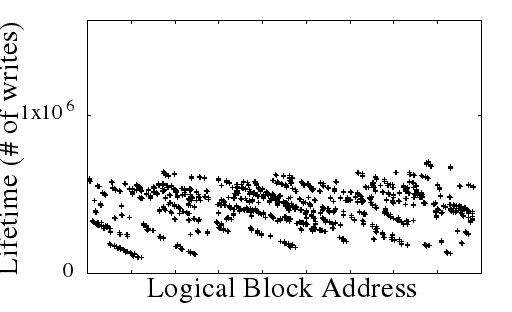
\includegraphics[width=0.4\textwidth]{figure/pcstream_/type_3}}
	\hspace{10pt}
	\subfloat[Flushing (manual)]{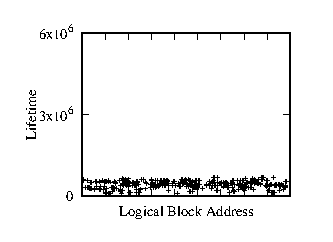
\includegraphics[width=0.4\textwidth]{figure/pcstream_/pcID_3}}
\caption{Data lifetime distributions of different PCs.} 
\label{fig:types_and_PCs_}
\end{figure}


In order to validate our hypothesis that PCs can be useful for estimating 
lifetimes by distinguishing dominant I/O activities, we conducted experiments
using RocksDB, comparing the accuracy of identifying dominant I/O activities
using two different methods.  First, we manually identified dominant I/O
activities by inspecting the source code. Second, we automatically decided
dominant I/O activities by extracting PCs for write-related system functions.
Fig.~\ref{fig:types_and_PCs_} illustrates two dominant I/O activities matched
between two methods.   As shown in Fig.~\ref{fig:types_and_PCs_}(a)
and~\ref{fig:types_and_PCs_}(b), the logging activity of RocksDB is correctly
identified by two methods.  Furthermore, from the logging-activity PC, we can
clearly observe that data written from the PC are short-lived. Similarly,
from Fig.~\ref{fig:types_and_PCs_}(c) and~\ref{fig:types_and_PCs_}(d), we observe
that data written from the flushing-activity PC behave in a different fashion.
For example, data from the flushing-activity PC remain valid a lot longer than
those from the logging-activity PC.

\section{Duplicate Data Patterns of I/O Activities}
\label{sec:duplicateactivity}
We analyzed the relationship between I/O activities and the duplicate data patterns of several applications
such as RocksDB and GCC.
Although it was difficult to find an I/O activity which is likely to have duplicate data,
we can find the relative difference in duplication rates (i.e., the percentage
of duplicate requests in total requests) for I/O activities for two reasons.

First, some activity reads and manipulates data stored in the device and write them, e.g., compaction 
activity of RocksDB.
Compaction activity merges multiple files which incurs 
reading multiple files from the device and writing them to the device after sorting.
If the key range is skewed, we may find untouched data sequence (same sequence as in read file)
after sorting.
The untouched data are regarded as duplicate data in the device.
Unlike compaction activity, the probability of finding duplicate data for logging and flushing activites is not very high
because data contents of logging and flushing activities are decided by users.
In summary, it is better to focus on compaction rather than logging and flushing to find duplicate data.

Second, activities with short-lived data are hard to be referenced, e.g., temporary files during compiling.
Most deduplication techniques work in the same way when duplicate data is not found.
As a regular write, an updated or trimmed page is invalidated.
However, the existing deduplication techniques for SSDs does not consider handling a fingerprint of an invalidated page.
The fingerprint value in the dedup table should be removed when the invalid page is erased.
We assume the fingerprint is removed right after the page invalidation because
removing all the fingerprints of invalid pages before erasing a block make GC overhead more severe.
Then, fingerprint of short-lived data can not stay long enough to be deduplicated.
In summary, we can avoid deduplication for PCs with short-lived data.

\begin{table}[b]
	\centering
	\begin{tabular}{c|c|c|c|c}
		\hline
		 \multirow{2}{*}{Application} & \multirow{2}{*}{I/O activity} & Duplicate & Total & Duplicate \\
									  &                               & requests  & requests & rate \\
		 \hline
		 \hline
		 \multirow{3}{*}{RocksDB} & logging & 0 & 39181 & 0\% \\
								  & flushing & 1092 & 102831 & 1\% \\
								  & compaction & 32201 & 398107 & 8\% \\
	     \hline
		 \multirow{2}{*}{GCC} & outputting & \multirow{2}{*}{0} & \multirow{2}{*}{193834} & \multirow{2}{*}{0\%} \\
							  & temp files &                    &                         & \\
		  \hline
	\end{tabular}
	\caption{Duplicate rates for I/O activities.}
	\label{tab:duprates}
\end{table}

In order to validate our analysis, we measured duplicate rate of aforementioned applications.
Table~\ref{tab:duprates} shows the duplicate rates of I/O activities for RocksDB and GCC. 
For RocksDB, Yahoo! Cloud Serving Benchmark (YCSB)~\cite{YCSB} with 
12-million keys was used to generate update-heavy workloads.
For GCC, a Linux kernel was built 30 times.  For each build, 1/3 of source files, which were
selected randomly, were modified and recompiled.
As explained, logging and flushing activities of RocksDB showed very low duplicate rates
while compaction activity shows higher duplicate rates.
Duplicate rate of outputting temporary file activity is also very low.
We can exploit this duplicate data patterns of I/O activities in designing 
an efficient deduplication technique.
